% Capítulo 8: Metodología
	\chapter{Metodología}\label{Cap: Metodología}
		\lipsum[1-4]. 
		\newpage
		The population mean $\mu$ is also called the \textit{expectation}
		of $X$, denoted $E(X)$ or sometimes simply $EX$. In general,
		the expectation of a function $g(X)$ is given by
		\begin{equation}
			E\left(g\left(X\right)\right) =
			\int\limits_{-\infty}^{\infty}g(x)f_{x}(x)dx,
		\end{equation}
		where $f_{x}(x)$ is the density of $X$. For example, the $r$th population moment of $X$ is the expectation of $X^{r}$.
		
		Consider the random variable $ a + bX$ for constants $a$ and $b$.
		Its expectation is 
		\begin{equation}
			\begin{aligned}
				E\left(a+bX\right) &= \int_{-\infty}^{\infty}
				\left[a + bx\right]\cdot f_{x}(x)dx \\
				&= a\int_{-\infty}^{\infty}f_{x}(x)dx  + 
				b\int_{-\infty}^{\infty}x\cdot f_{x}(x)dx\\
				&= a + bE(X)
			\end{aligned}
		\end{equation}
		\lipsum[1]
		\begin{equation}\label{eq: MLG}
			Y_{i} = \beta_{1} + \beta_{2}X_{2i} + \cdots + \beta_{k}X_{ki} + \mu_{i}
		\end{equation}
		\lipsum[1]
		\begin{figure}[h!]
			\centering
			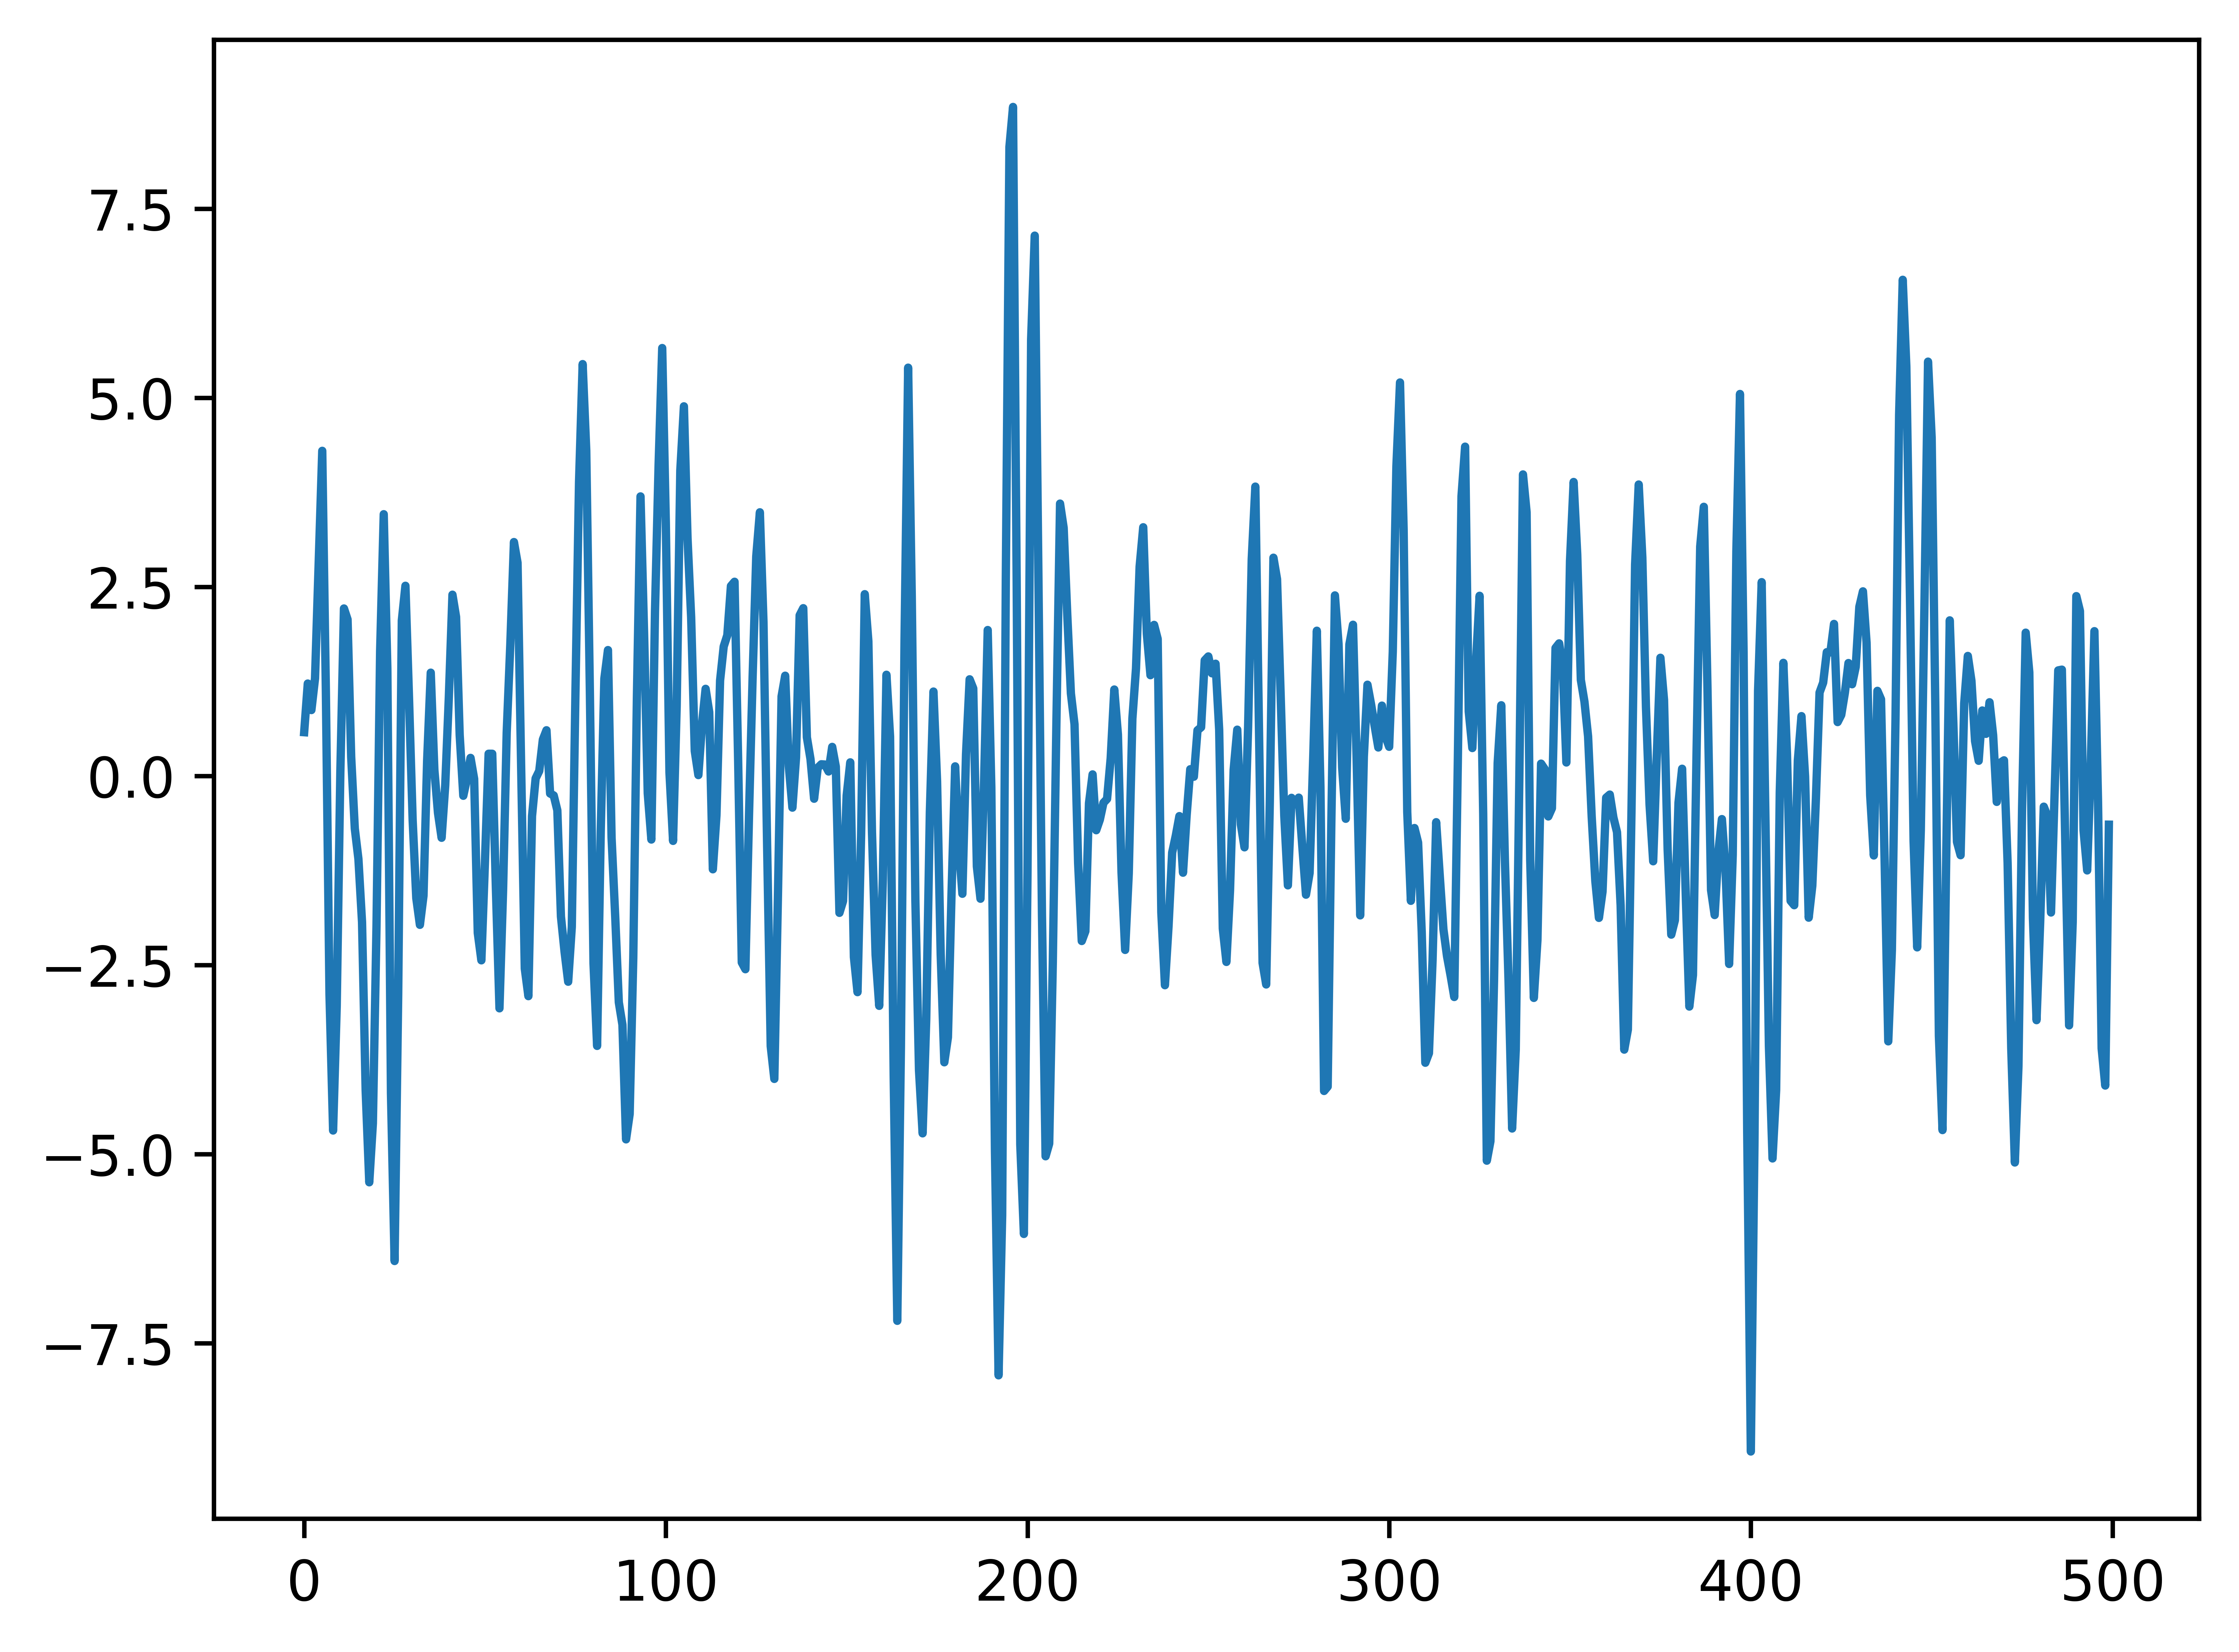
\includegraphics[height=7cm]{Graph1.png}
			\caption{Graph1}
			\label{fig: Graph1}
		\end{figure}
		\lipsum[1] 
		\vspace{0.7cm}\\
		\textcolor{red!75}{Equivalence between DC and SE}. Under usual
		regularity conditions (convexity and Inada conditions), and given
		$b^{i}(s^{0}) = \text{for all} \quad i \in I$, the allocations of the Debreu
		competitive equilibrium and the allocations of the sequential equilibrium
		are equivalent. Moreover, the spence of wages and interest rates are the same, and
		\begin{equation}\label{eq: DC and SE}
			Q(s^{t+1}|s^{t}) = \frac{q(s^{t+1})}{q(s^{t})} =
			\beta \frac{U_{c}^{i}(s^{t+1})}{U_{c}^{i}(s^{t})} \frac{\pi(s^{t+1})}{\pi(s^{t})}
		\end{equation}
		for all $ t, s^{t}$, and $s^{t+1}|s^{t}$.
		% Sección 8.1: Tipo y Nivel de Investigación
			\section{Tipo y Nivel de Investigación}\label{Sec: Tipo y Nivel de Investigación}
				\lipsum[1]. Como se muestra el la ecuación \textcolor{blue}{\eqref{eq: MLG}}
				\begin{figure}[h!]
					\centering
					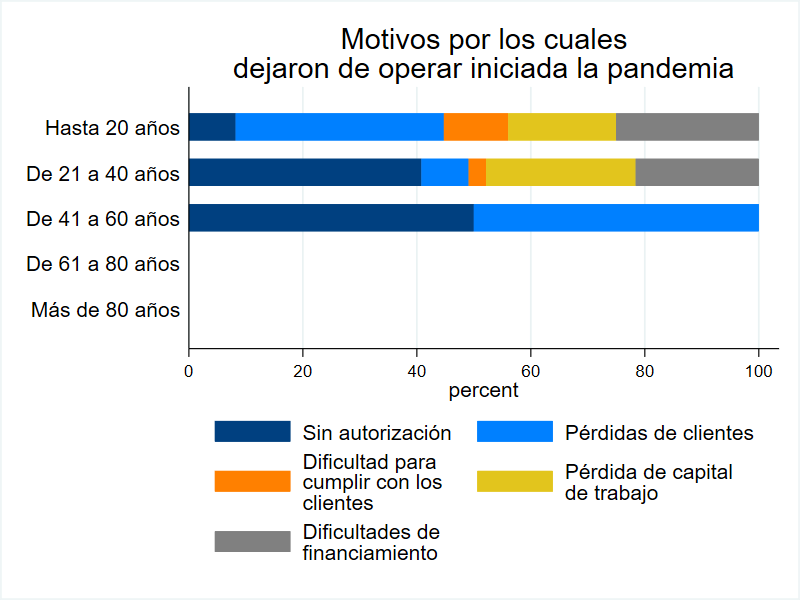
\includegraphics[height=7cm]{Graph2.png}
					\caption{Graph2}
					\label{fig: Graph2}
				\end{figure}
		% Sección 8.2: Población y Muestra 
			\section{Población y Muestra}\label{Sec:Población y Muestra}
				\lipsum[1]. Como se muestra en la ecuación \textcolor{blue}{\eqref{eq: DC and SE}}. Asimismo, las figuras que se muestran a continuación fueron extraidos de \textcolor{blue}{\cite{Huang-2022}}.
				\begin{figure}[h!]
					\centering
					\begin{subfigure}[b]{0.3\textwidth}
						\centering
						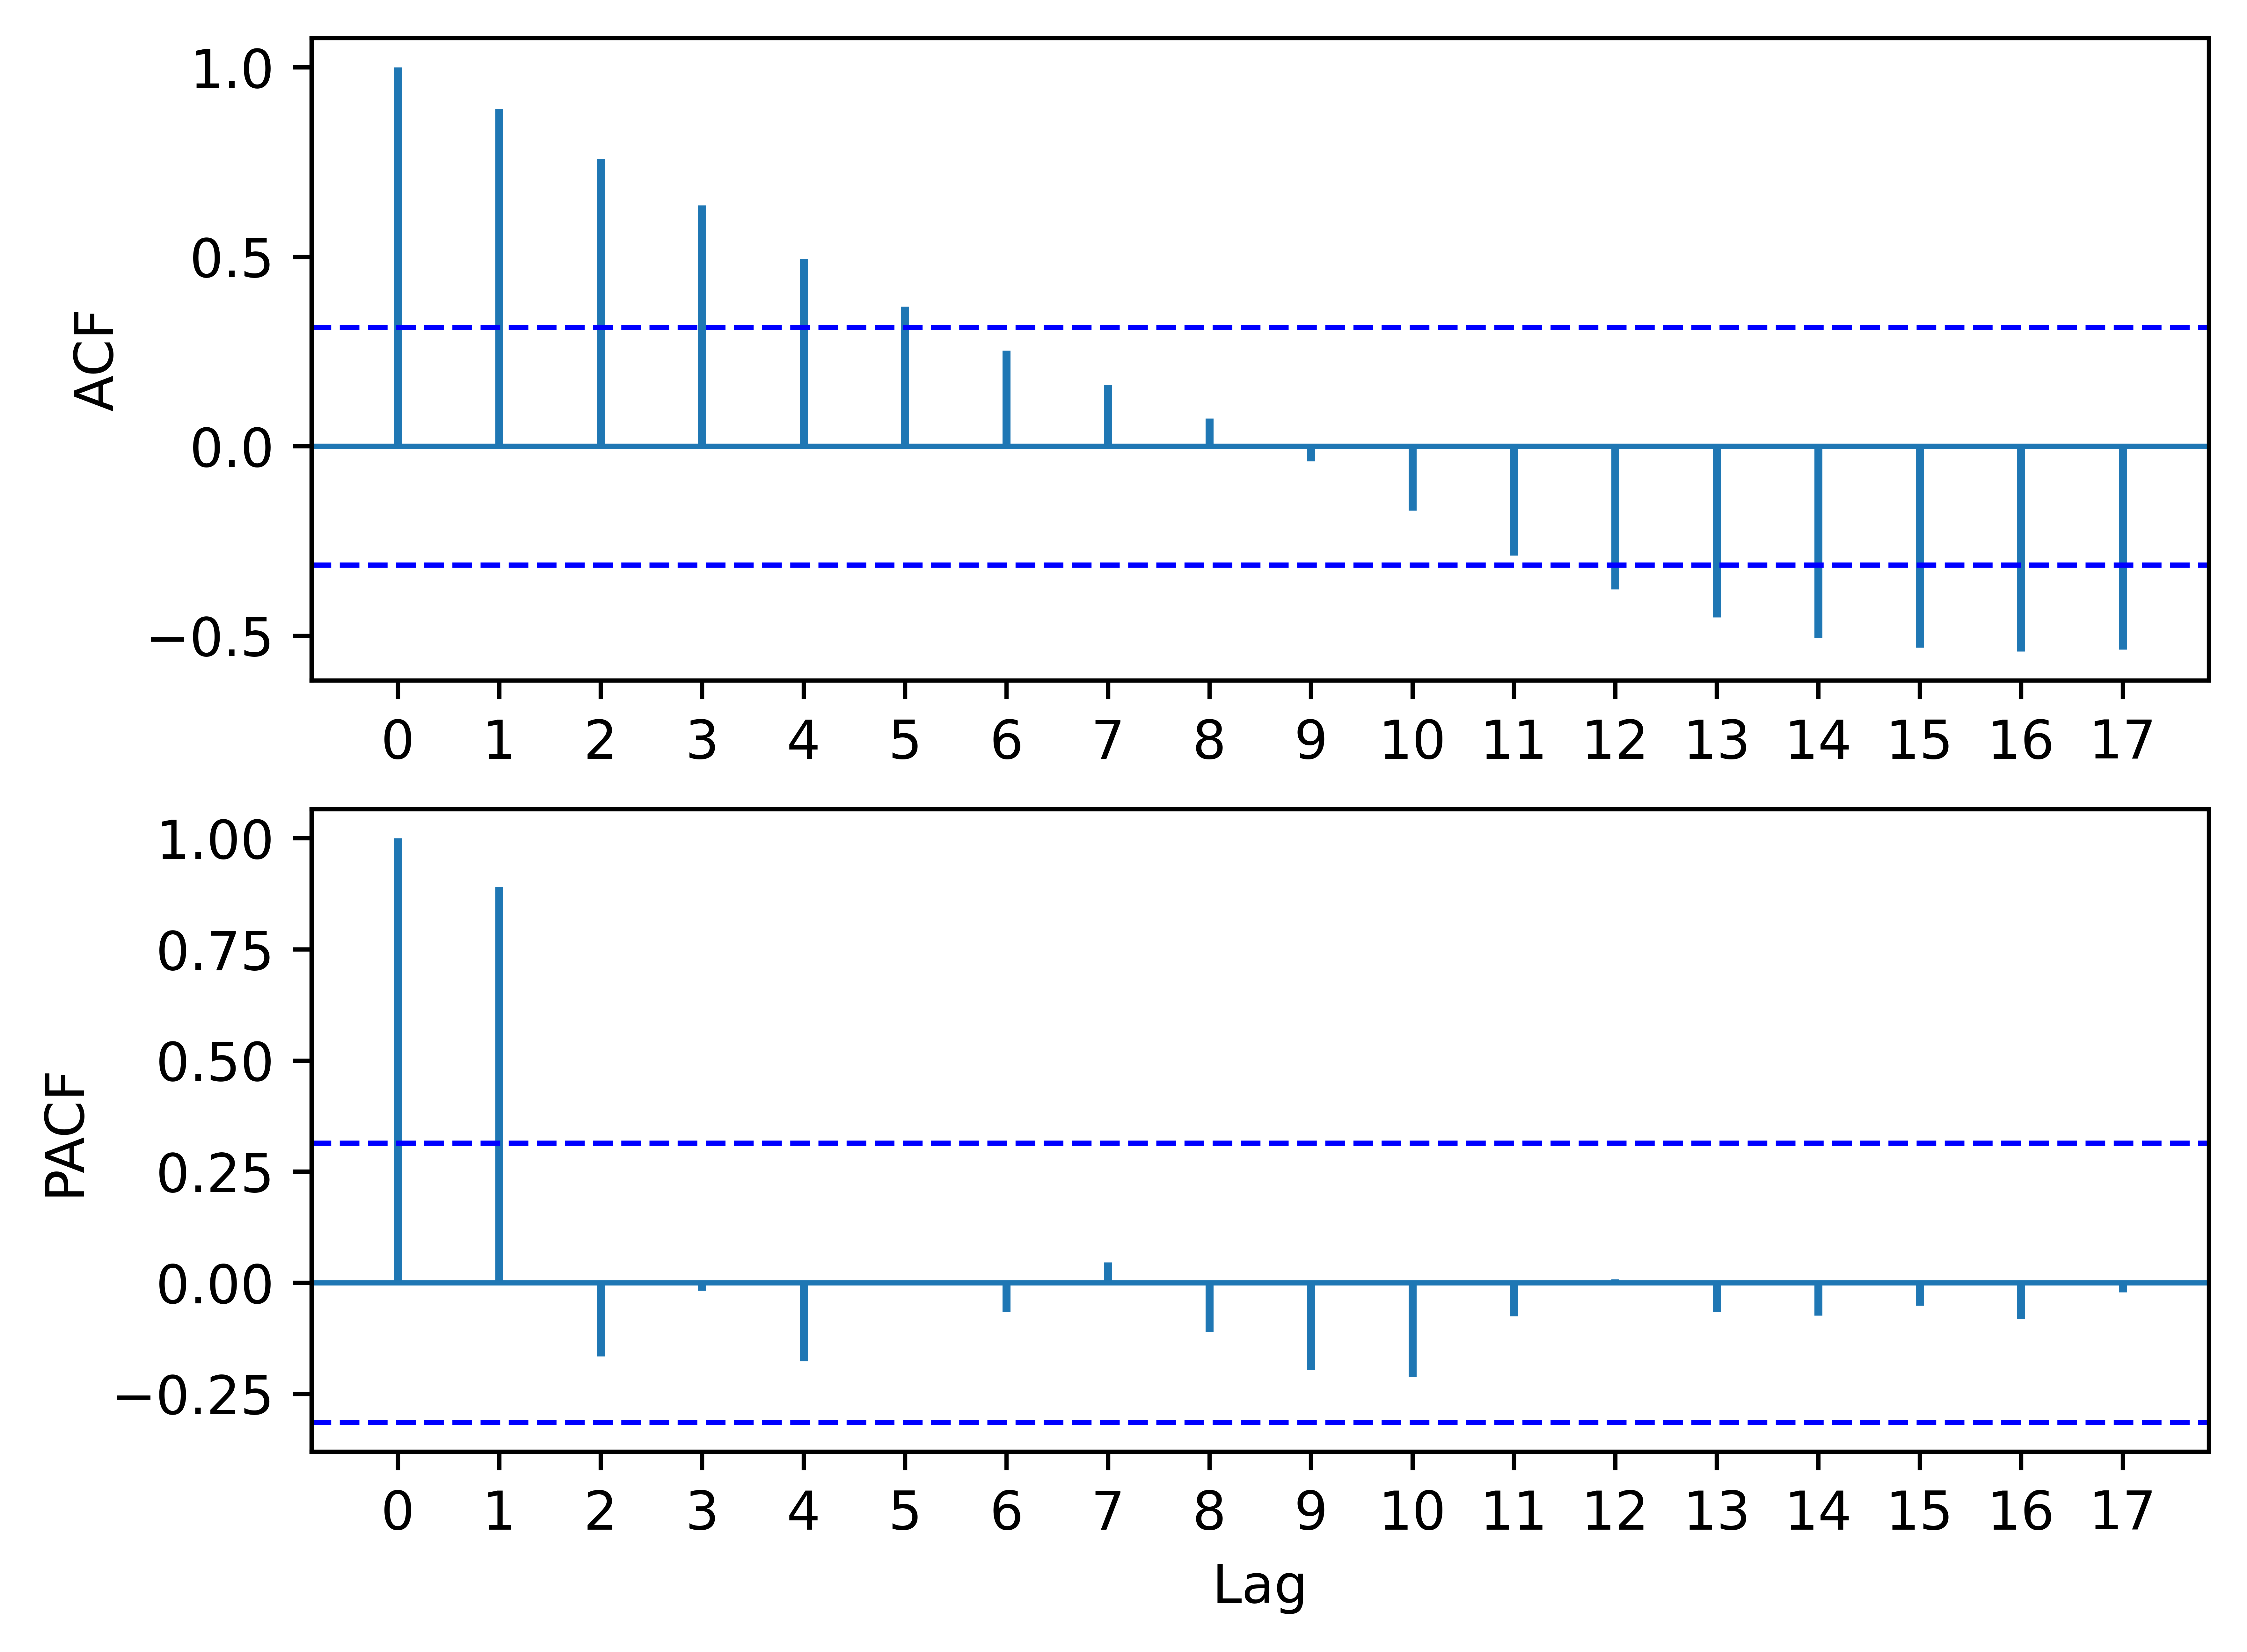
\includegraphics[width=\textwidth]{Graph6.png}
						\caption{Graph6}
						\label{subfig: Graph6}
					\end{subfigure}
					\hfill
					\begin{subfigure}[b]{0.3\textwidth}
						\centering
						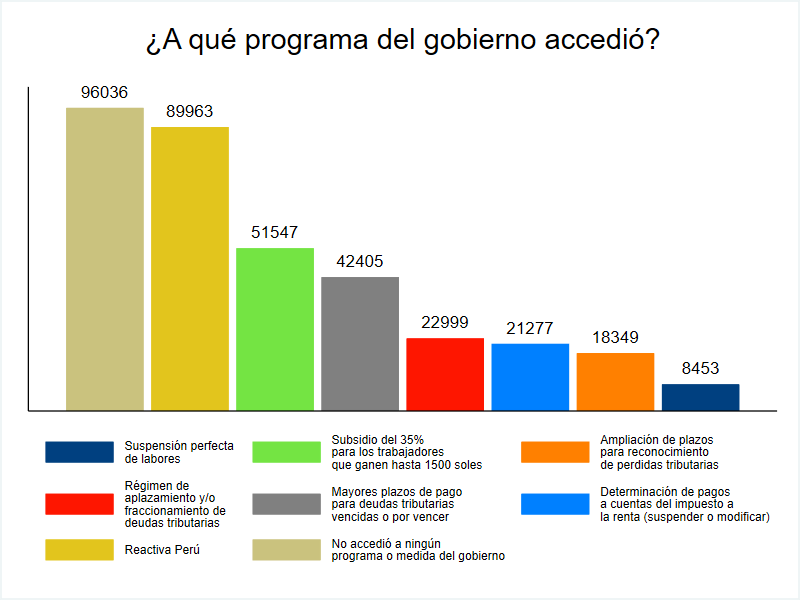
\includegraphics[width=\textwidth]{Graph4.png}
						\caption{Graph4}
						\label{subfig: Graph4}
					\end{subfigure}
					\hfill
					\begin{subfigure}[b]{0.3\textwidth}
						\centering
						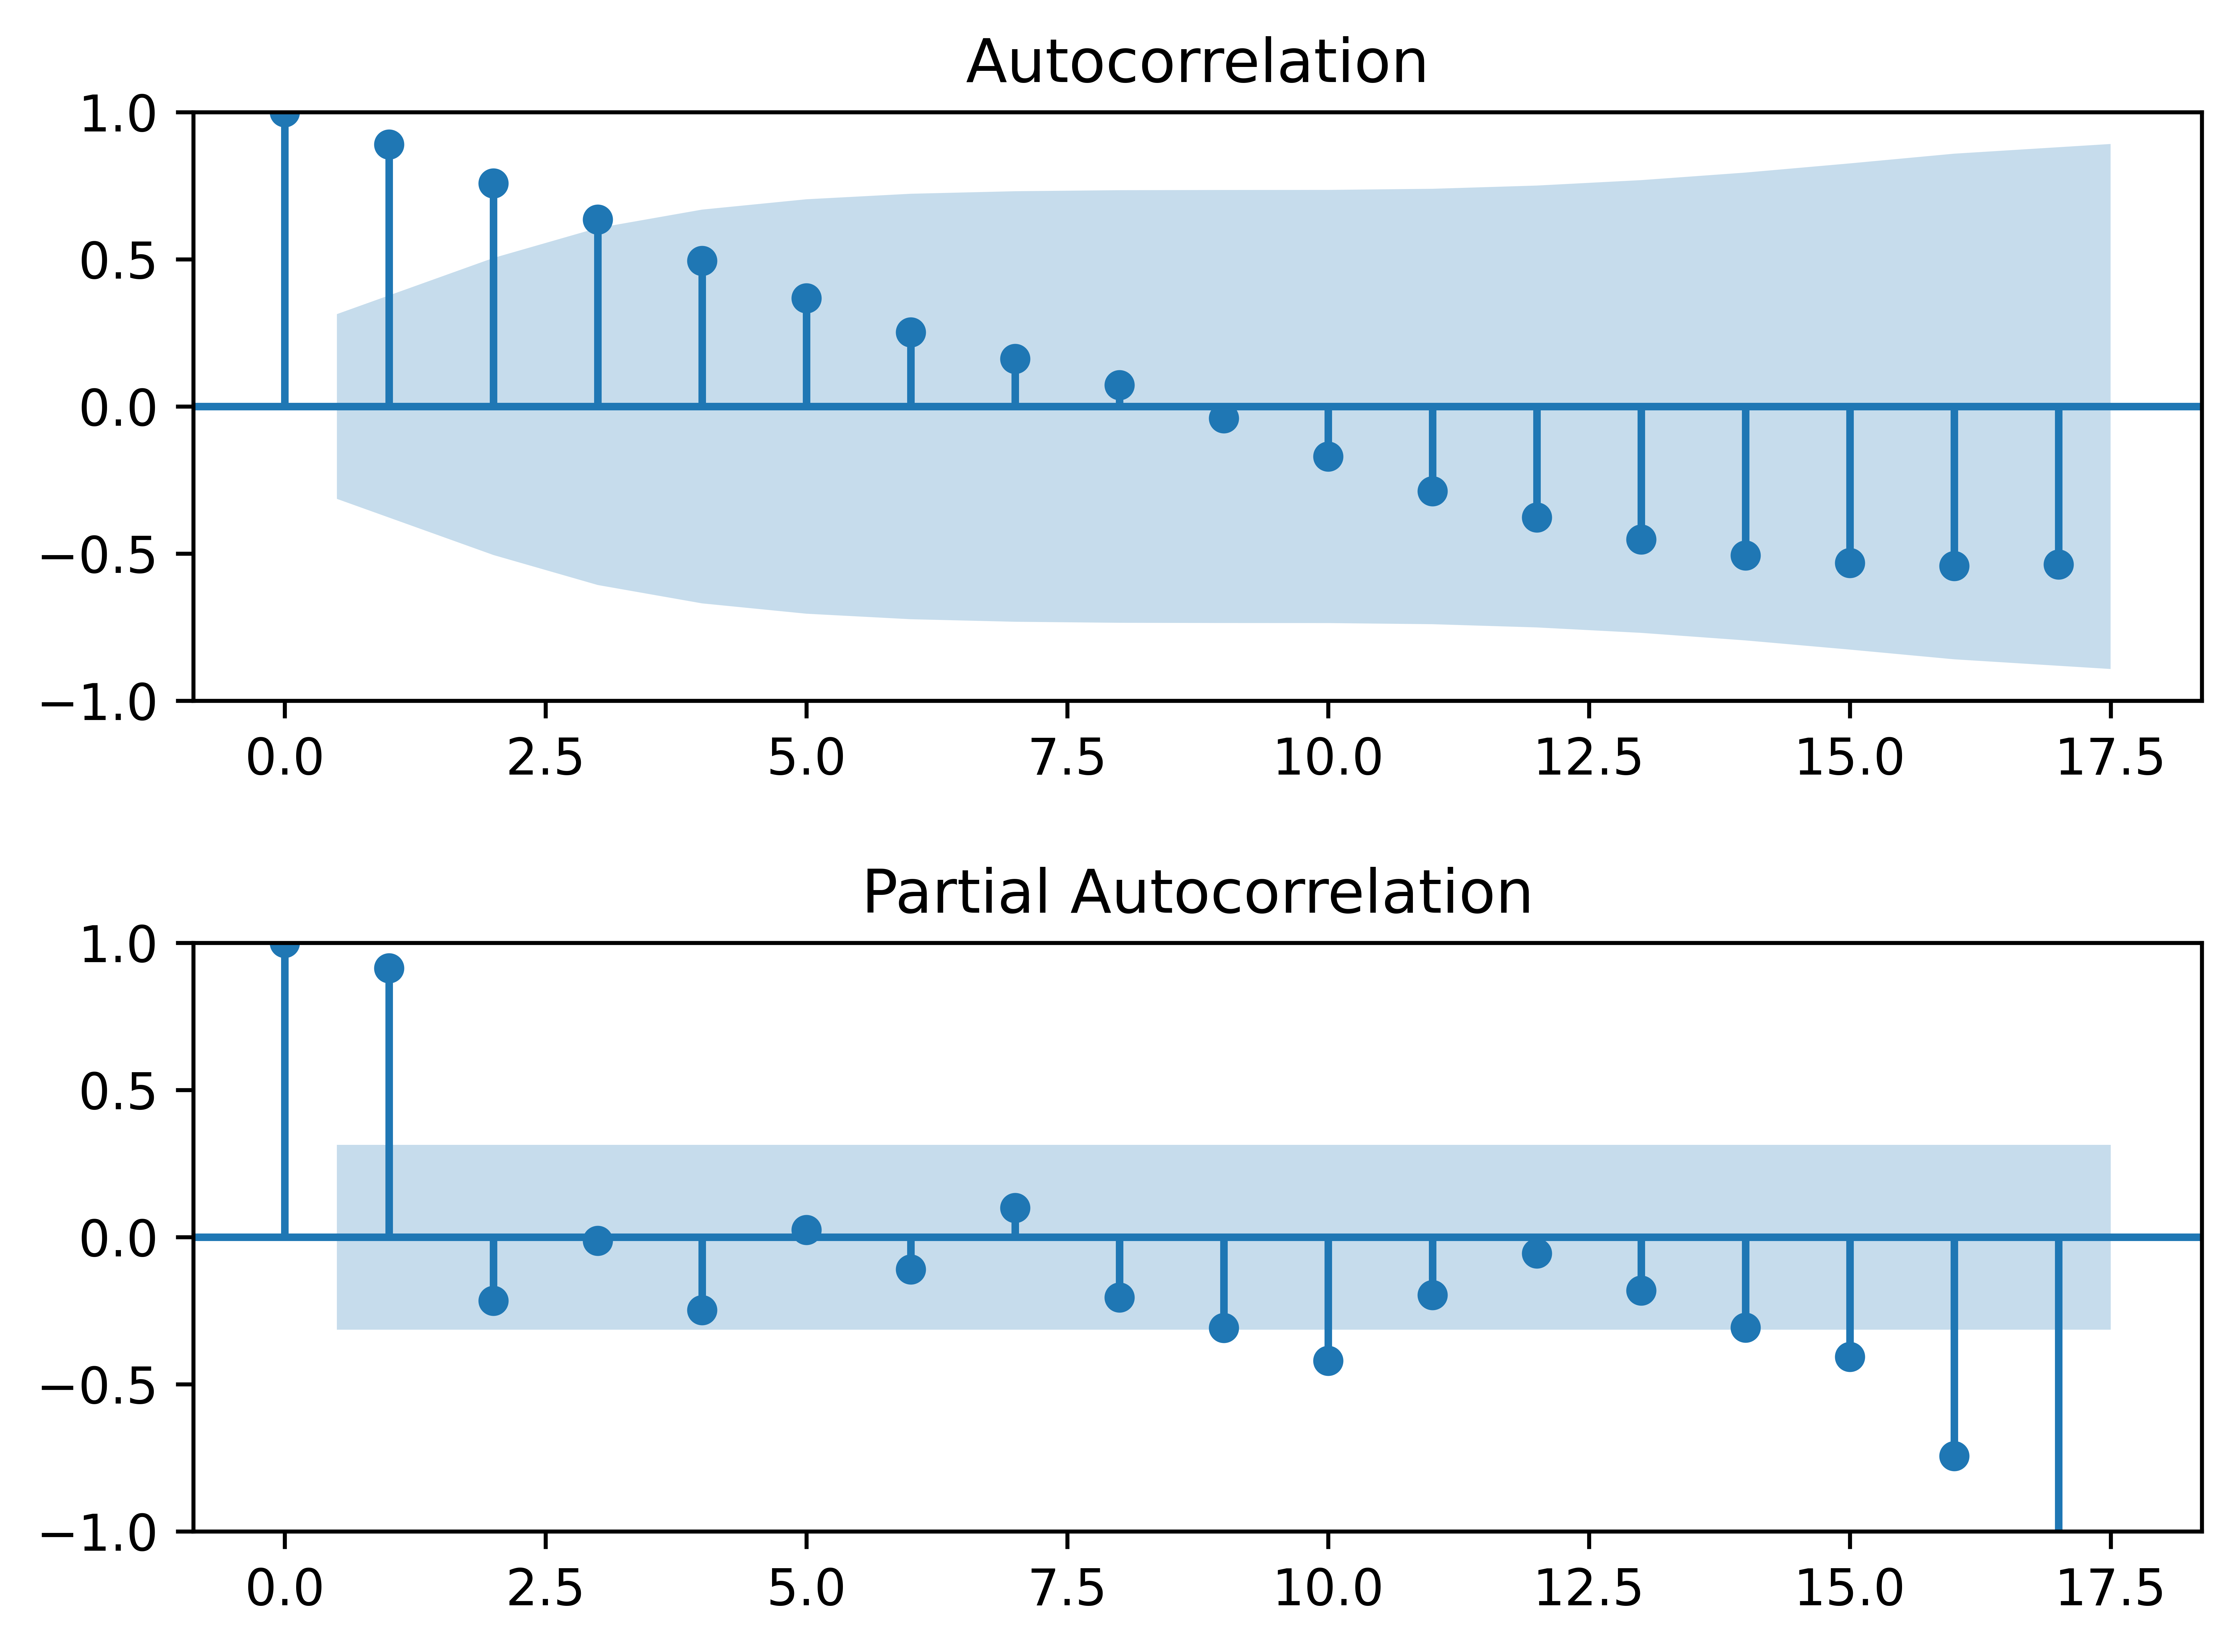
\includegraphics[width=\textwidth]{Graph5.png}
						\caption{Graph5}
						\label{subfig: Graph5}
					\end{subfigure}
					\caption{Graficas multiples}
					\label{fig: Graficas multiples}
				\end{figure}
		% Sección 8.3: Fuentes de Información
			\section{Fuentes de Información}\label{Sec: Fuentes de Información}
				\lipsum[1]
				\begin{figure}[ht]
					\centering
					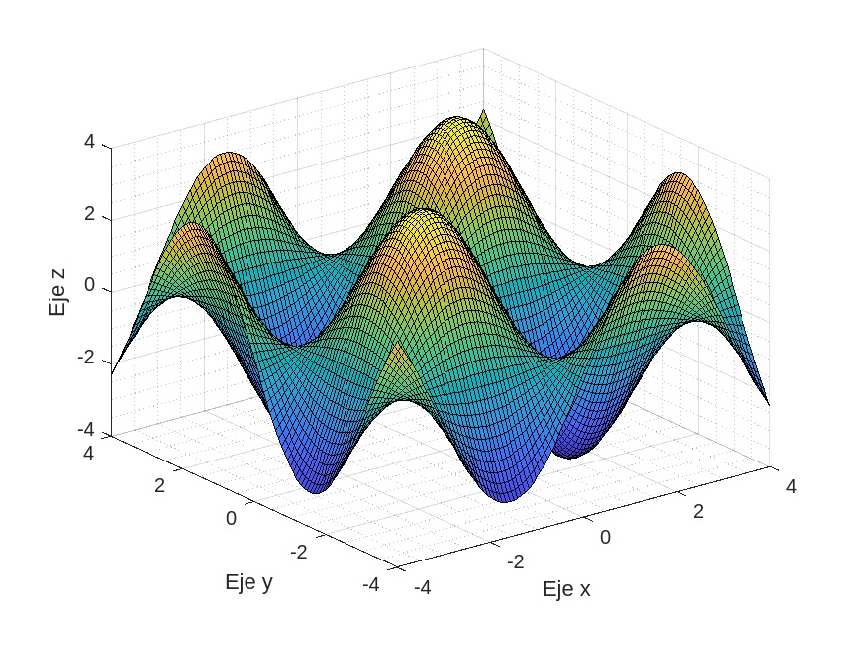
\includegraphics[height=7cm]{Graph3D.pdf}
					\caption{Graph3D}
					\label{fig: Graph3D}
				\end{figure}
		% Sección 8.4: Diseño de Investigación
			\section{Diseño de Investigación}\label{Sec: Diseño de Investigación}
				\lipsum[1]
				\begin{figure}[ht]
					\centering
					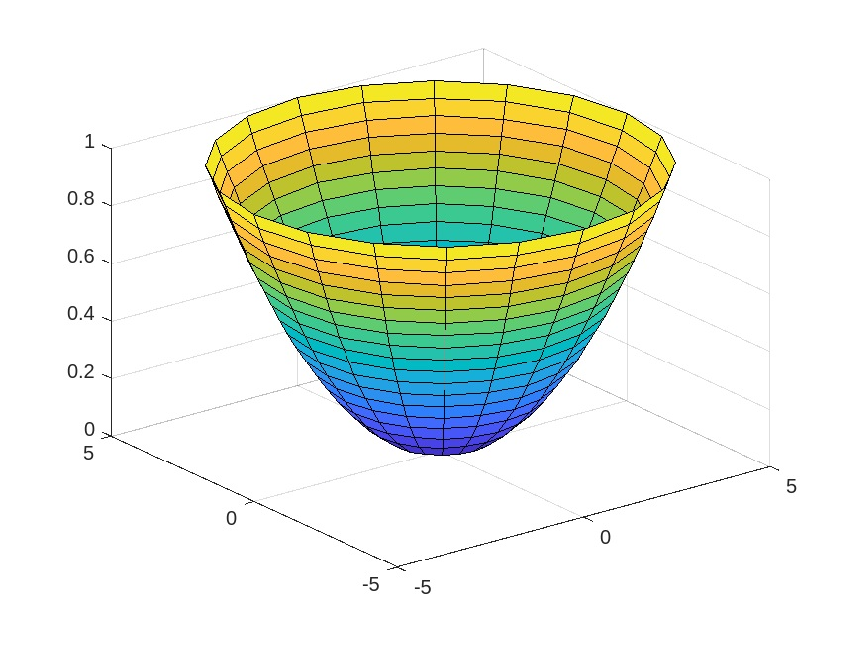
\includegraphics[height=7cm]{Graph3D_2.pdf}
					\caption{Graph3D-2}
					\label{fig: Graph3D-2}
				\end{figure}
		% Sección 8.5: Téncicas e Intrumentos 
			\section{Téncicas e Intrumentos }\label{Sec: Téncicas e Intrumentos }
				\lipsum[1]
				\begin{figure}[H]
					\centering
					\begin{tikzpicture}[scale = 1.8, samples = 70]
						\fill[green] (0,0) -- plot[domain = 0:pi] ({\x}, {sin(\x r)}) -- (pi,0) -- cycle;
						\fill[green] (pi,0) -- plot[domain = pi:2*pi] ({\x}, {sin(\x r)}) -- (2*pi,0) -- cycle;
						\draw[dashed, xstep = pi/2] (-pi/4, -1) grid (9*pi/4, 1);
						\draw[<-] (7,0) node[below right] {$x$} -- (-0.5,0); 
						\draw[<-] (0,1.25) node[above left] {$y$} -- (0, -1.25); 
						\node[below right] at (pi/2, 0) {$\frac{\pi}{2}$};
						\node[below right] at (pi, 0) {$\pi$};
						\node[below right] at (3*pi/2, 0) {$\frac{3\pi}{2}$};
						\node[below right] at (2*pi, 0) {$2\pi$};	
						\node[left] at (0,1) {$1$};
						\node[left] at (0,-1) {$-1$};
						\draw[very thick, azul, domain = -0.5 + 0:2*pi + 0.5] plot({\x}, {sin(\x r)}) node[right] {$h(x) = \sin x$};
						\draw[very thick, red, domain = -0.5 + 0:2*pi + 0.5] plot({\x}, {cos(\x r)}) node[above] {$g(x) = \cos x$};
					\end{tikzpicture}
					\caption{Función seno y coseno}
					\label{fig: Función seno}
				\end{figure}
				\lipsum[1].
				\begin{equation}\label{eq: NL1}
					\alpha_{n}b_{n+1} + \beta_{n}b_{n} + \gamma_{n}b_{n-1} + \delta_{n}b_{n-2} +\varepsilon_{n}b_{n-3} = 0
				\end{equation}
				donde,
				\begin{eqnarray}
					\alpha_{n} &=& \left(n+1\right)\left(n+1+|m|\right), \label{eq: NL2}\\
					\beta_{n} &=& -2n\left(2n+|m|\right) + m^{2}+|m| + k + \dfrac{a_{0}\in^{2}}{\ell^{2}}+\dfrac{2}{\ell}, \label{eq: NL3}\\
					\gamma_{n} &=& 6(n-1)^{2}-2\left(m^{2} + |m| + k + \dfrac{a_{0}^{2}\in^{2}}{\ell^{2}}\right), \label{eq: NL4} \\
					\delta_{n} &=& 2(n-2)\left(|m| - 2n + 4\right) + m^{2} + |m| + k + \dfrac{a_{0}\in^{2}}{\ell^{2}}-\dfrac{2}{\ell}, \label{eq: NL5}\\
					\varepsilon_{n} &=& (n-3)\left(n-3-|m|\right), \label{eq: NL6}
				\end{eqnarray}
				Estos resultados se pueden ver en \cite{Kim-2008}